\pagebreak

\section{Simulation Analysis}
\label{sec:simulation}

\paragraph{}
In this section, we can find the results of the topics required in the simulation analysis. The numeric results or graphics are presented alongside a short explanation of the interpretation of the problem. All of the results were obtained using NGSpice and the section is divided in three different subsections. 

\subsection{Output Voltage Gain}

\paragraph{}
The output stage of the common collector amplifier allows the circuit to be compatible with the speaker impedance limits. It is possible to analyse the output voltage of this second part of the amplifier circuit relating it with the variation of the frequency. The NGSpice analysis results in the plot shown below.


\begin{figure}[H]\centering
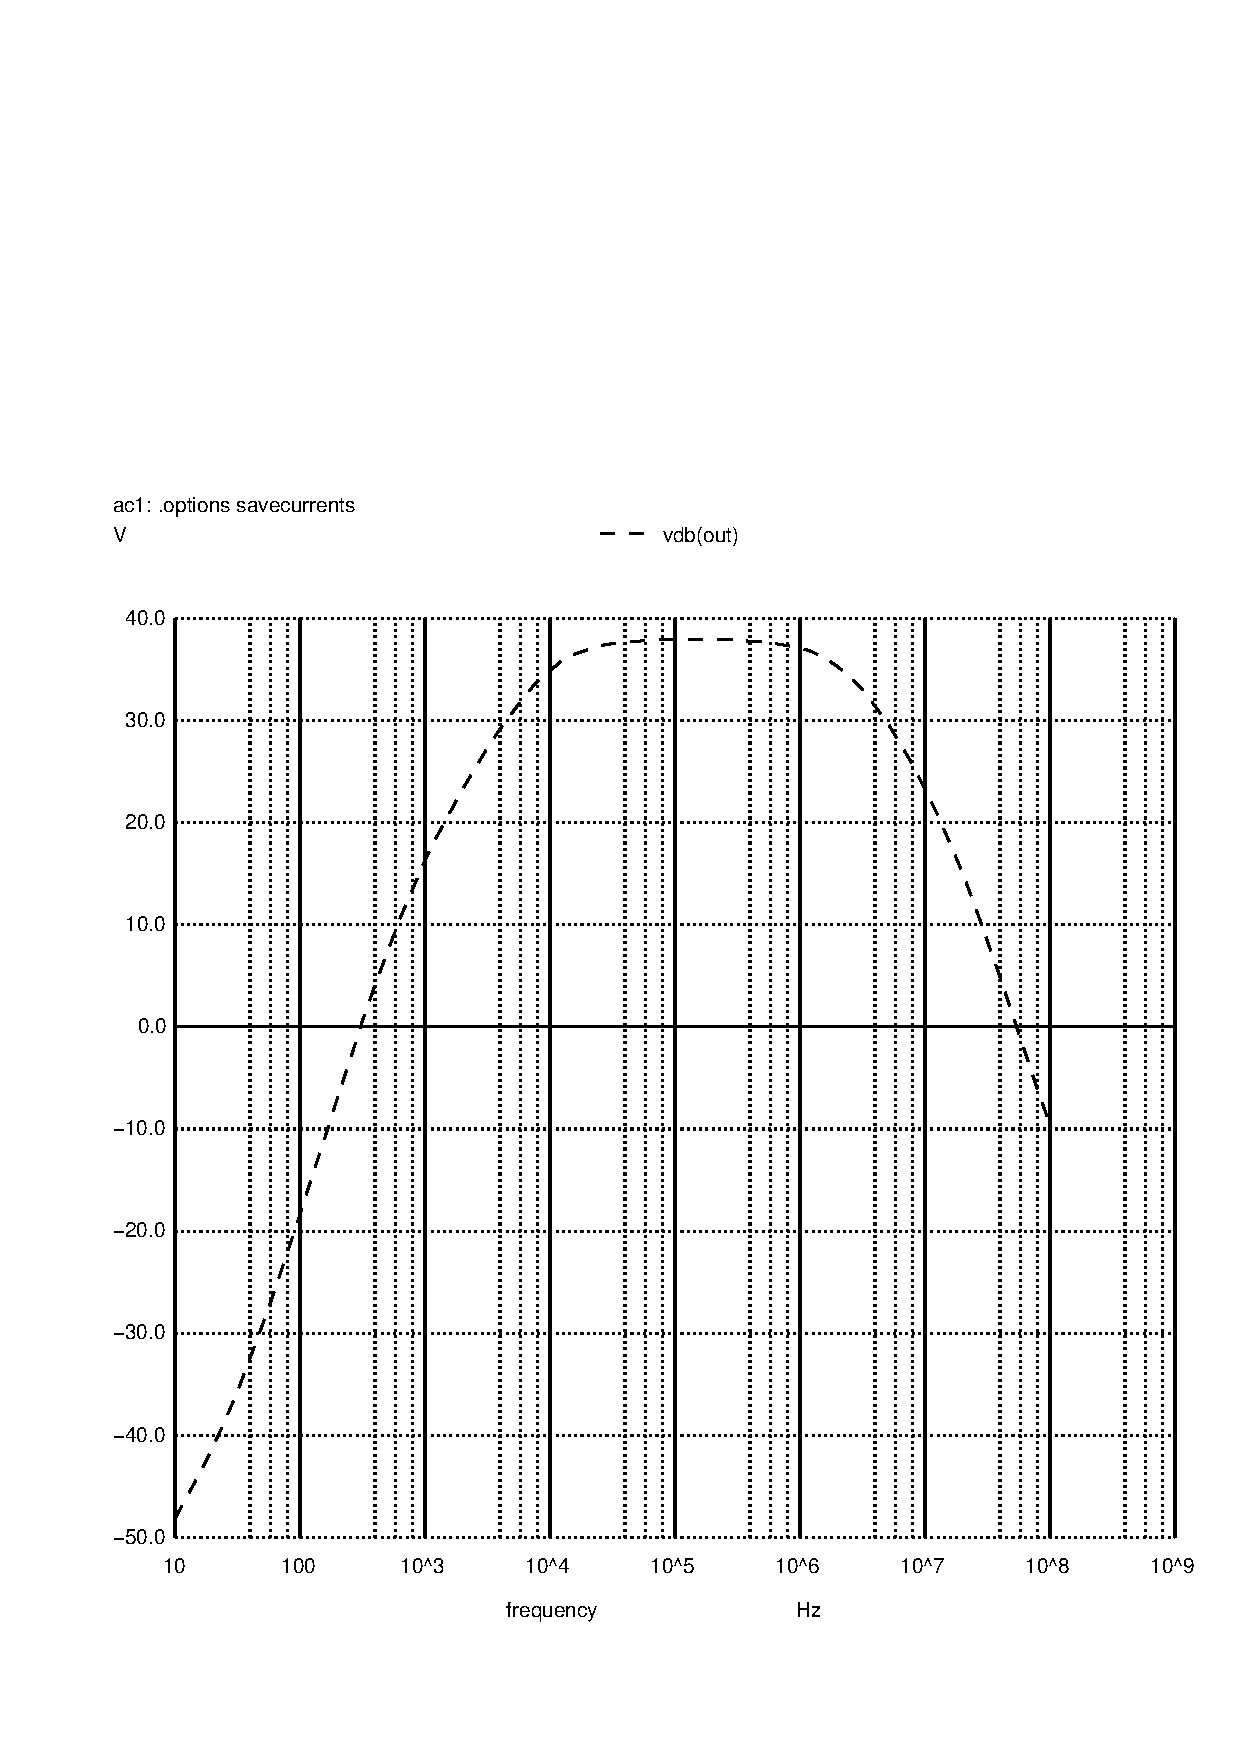
\includegraphics[trim= 0cm 0cm 0cm 10cm, clip, width=0.7\textwidth]{vo2f.pdf}
\caption{The Output Voltage of the Output Stage of a Common Collector Amplifier.}
\label{fig:sim_output}
\end{figure}

where $f$ is expressed in Hertz (Hz) along the x-axis\\
and $v_{dB_{out}}$, the output voltage of the amplifier, is expressed in  in Volts (V) using a decibel scale along y-axis.

\paragraph{}
The interpretation of the graphic allows us to see that the output voltage tends to become constant when closer to its maximum values. In fact, it is possible to compute the output voltage gain as an approximation of the maximum output voltage level.


\begin{table}[H] \centering
  \begin{tabular}{|l|r|}
    \hline    
    {\bf NGSpice Formula} & {\bf Output Voltage Gain (V)} \\ \hline
    \input{outvoltagegain_TAB}
  \end{tabular}
 \label{tab:outvoltagegain}
\end{table}

%%%%%

\subsection{Bandwidth and Cut-Off Frequencies}

\paragraph{}
Also from the intepretation of the plot presented in the previous usbsection, we can calculate the cut-off frequencies. In this case, since we are using an electric circuit simulation tool like NGSpice, we are able to compute values for two existing cut-off frequencies. They are calculated as 3dB cut off frequencies, which means that their correspondent output voltage is the same and it is 3dB lower than the maximum output voltage level. From the lower and upper cut-off frequencies it is possible to calculate the bandwidth. 

\begin{table}[H] \centering
  \begin{tabular}{|l|r|}
    \hline    
    {\bf Variable} & {\bf Frequency Value (Hz)} \\ \hline
    \input{cutofffreq_TAB}
  \end{tabular}
 \label{tab:cutofffreq}
\end{table}

where $f_1$ is the lower cut-off frequency,\\
a$f_1$ is the upper cut-off frequency and\\
$f_2-f_1$ is the bandwith (the difference between the upper and lower cut-off frequencies).

%%%%%

\subsection{Input and Output Impedances}

\paragraph{}
The impedances of the common collector amplifier are really important values to obtain when trying to interpretate the viability of the amplifier circuit. And that's why it is really important to calculate the input impedance and the output impedance for both the gain and output stages of the amplifier. After all the values are computed, the circuit can be approved as a common colector amplifier if all the impedances are within the limits allowed by the driver (input audio source) and the load (speaker).

\paragraph{}
The following values were obtained using different NGSpice circuits built specifically to calculate each one of the impedances. Alternate voltage sources with different parameters were used in order to aplly the Ohm's law with impedances and compute the impedance for each case studied. In both output stage's impedances and also in the output impedance of the gain stage, an auxiliary capacitor was applyed to the circuits  in series with the voltage source in order to cancel the DC variations of the circuit and get a straight analysis exclusively from sinusoidal components.

\begin{table}[H] \centering
  \begin{tabular}{|l|r|}
    \hline    
    {\bf NGSpice Formula} & {\bf Gain Stage Input Impedance ($\Omega$): $a,b$ from $Z_{in}=a+bj$}\\ \hline
    \input{inputimpgain_TAB}
  \end{tabular}
 \label{tab:inputimp}
\end{table}

\begin{table}[H] \centering
  \begin{tabular}{|l|r|}
    \hline    
    {\bf NGSpice Formula} & {\bf Gain Stage Output Impedance ($\Omega$)}\\ \hline
    \input{outimpgain_TAB}
  \end{tabular}
 \label{tab:outimp}
\end{table}

\begin{table}[H] \centering
  \begin{tabular}{|l|r|}
    \hline    
    {\bf NGSpice Formula} & {\bf Output Stage Input Impedance ($\Omega$)}\\ \hline
    \input{inputimpoutput_TAB}
  \end{tabular}
 \label{tab:inputimp2}
\end{table}

\begin{table}[H] \centering
  \begin{tabular}{|l|r|}
    \hline    
    {\bf NGSpice Formula} & {\bf Output Stage Output Impedance ($\Omega$)}\\ \hline
    \input{outimpoutput_TAB}
  \end{tabular}
 \label{tab:outimp2}
\end{table}


\pagebreak
